\documentclass[UTF8,zihao=-4]{ctexart}
\usepackage[a4paper,margin=1.8cm]{geometry}
\usepackage{longtable,booktabs,array,graphicx,float,hyperref,listings}
\setCJKmainfont{SimSun}
\setCJKsansfont{Microsoft YaHei}
\setmainfont{Times New Roman}
\hypersetup{colorlinks=true,linkcolor=blue,urlcolor=blue}
\lstset{basicstyle=\ttfamily\scriptsize,breaklines=true,frame=single,columns=fullflexible}
\newcolumntype{P}[1]{>{\raggedright\arraybackslash}p{#1}}
\title{软件系统综合课程设计——练习1（黑盒+功能测试）\\西南交通大学校园论坛系统测试报告}
\author{测试人员：课程设计小组成员}
\date{2026年6月9日}
\begin{document}
\maketitle
\tableofcontents
\newpage

\section{项目名称、简介与测试范围}
项目名称为“西南交通大学校园论坛系统”。被测对象为便携运行包\texttt{swjtu-forum-portable}，前端运行在4173端口，后端运行在8080端口，demo profile使用H2本地数据库。本轮根据最新要求每个功能点保留5条高价值测试用例，共75条，删除低优先级、未验证和IE兼容设计类用例，优先保留已经执行、有截图证据或可由接口自动化稳定验证的用例。

\section{功能点清单}
\begin{longtable}{P{1cm}P{3cm}P{6cm}P{2cm}}
\toprule
序号 & 一级功能 & 二级功能 & 用例数\\
\midrule
\endfirsthead
\toprule
序号 & 一级功能 & 二级功能 & 用例数\\
\midrule
\endhead
1 & 用户注册 & 新用户注册 & 5 \\
2 & 用户登录 & 账号密码登录 & 5 \\
3 & 帖子浏览 & 首页帖子列表 & 5 \\
4 & 帖子浏览 & 按版块筛选帖子 & 5 \\
5 & 帖子浏览 & 帖子搜索 & 5 \\
6 & 发帖 & 发布新帖子 & 5 \\
7 & 评论 & 发表评论 & 5 \\
8 & 互动 & 点赞帖子 & 5 \\
9 & 互动 & 收藏帖子 & 5 \\
10 & 个人中心 & 编辑个人资料 & 5 \\
11 & 个人中心 & 校园身份认证 & 5 \\
12 & 成长系统 & 每日签到 & 5 \\
13 & 积分商城 & 积分兑换奖品 & 5 \\
14 & 通知中心 & 查看通知 & 5 \\
15 & 关注 & 关注/取消关注用户 & 5 \\
\bottomrule
\end{longtable}

\section{测试方法与执行策略}
本报告仍以黑盒测试为主，方法包括等价类划分、边界值分析和判定表。压缩后每个功能点只保留5条高价值用例：一条正常主流程、一到两条边界/异常、一条未登录或状态迁移、一条页面或截图验证。这样既满足课程要求中的关键路径覆盖，又避免把大量没有实际执行价值的低优先级设计项塞进报告。

执行上采用“接口自动化优先，Selenium验证关键UI”的方式。接口自动化覆盖注册、登录、帖子列表、版块筛选、搜索、发帖、评论、点赞、收藏、资料编辑、校园认证、签到、积分兑换、通知和关注；Selenium/Chrome负责页面展示、按钮点击、通知中心展开、积分商城刷新和移动端截图。IE/Edge IE模式未配置真实环境，因此相关低优先级兼容项已删除，不写成通过。

\section{测试环境}
\begin{itemize}
\item 操作系统：Windows。
\item 后端：Spring Boot便携jar，端口8080。
\item 前端：frontend-server.jar，端口4173。
\item 浏览器：Google Chrome，桌面视口1440×1000，移动端视口390×844。
\item 自动化：批量HTTP接口脚本、Selenium WebDriver + JUnit 5。
\item 报告编译：XeLaTeX，TeX源文件位于课程设计模板目录。
\end{itemize}

\section{功能点逐项分析}
\subsection{1. 用户注册：新用户注册}
用户注册的新用户注册保留5条高价值用例，删除了低优先级IE兼容、极端空数据和重复设计项。保留项覆盖正常路径、边界/异常、未登录权限、刷新后状态和关键UI证据。该功能点的执行结果由批量HTTP接口脚本、Selenium/JUnit脚本和Chrome截图共同支撑，因此报告中不再保留大面积未验证条目。

\subsection{2. 用户登录：账号密码登录}
用户登录的账号密码登录保留5条高价值用例，删除了低优先级IE兼容、极端空数据和重复设计项。保留项覆盖正常路径、边界/异常、未登录权限、刷新后状态和关键UI证据。该功能点的执行结果由批量HTTP接口脚本、Selenium/JUnit脚本和Chrome截图共同支撑，因此报告中不再保留大面积未验证条目。

\subsection{3. 帖子浏览：首页帖子列表}
帖子浏览的首页帖子列表保留5条高价值用例，删除了低优先级IE兼容、极端空数据和重复设计项。保留项覆盖正常路径、边界/异常、未登录权限、刷新后状态和关键UI证据。该功能点的执行结果由批量HTTP接口脚本、Selenium/JUnit脚本和Chrome截图共同支撑，因此报告中不再保留大面积未验证条目。

\subsection{4. 帖子浏览：按版块筛选帖子}
帖子浏览的按版块筛选帖子保留5条高价值用例，删除了低优先级IE兼容、极端空数据和重复设计项。保留项覆盖正常路径、边界/异常、未登录权限、刷新后状态和关键UI证据。该功能点的执行结果由批量HTTP接口脚本、Selenium/JUnit脚本和Chrome截图共同支撑，因此报告中不再保留大面积未验证条目。

\subsection{5. 帖子浏览：帖子搜索}
帖子浏览的帖子搜索保留5条高价值用例，删除了低优先级IE兼容、极端空数据和重复设计项。保留项覆盖正常路径、边界/异常、未登录权限、刷新后状态和关键UI证据。该功能点的执行结果由批量HTTP接口脚本、Selenium/JUnit脚本和Chrome截图共同支撑，因此报告中不再保留大面积未验证条目。

\subsection{6. 发帖：发布新帖子}
发帖的发布新帖子保留5条高价值用例，删除了低优先级IE兼容、极端空数据和重复设计项。保留项覆盖正常路径、边界/异常、未登录权限、刷新后状态和关键UI证据。该功能点的执行结果由批量HTTP接口脚本、Selenium/JUnit脚本和Chrome截图共同支撑，因此报告中不再保留大面积未验证条目。

\subsection{7. 评论：发表评论}
评论的发表评论保留5条高价值用例，删除了低优先级IE兼容、极端空数据和重复设计项。保留项覆盖正常路径、边界/异常、未登录权限、刷新后状态和关键UI证据。该功能点的执行结果由批量HTTP接口脚本、Selenium/JUnit脚本和Chrome截图共同支撑，因此报告中不再保留大面积未验证条目。

\subsection{8. 互动：点赞帖子}
互动的点赞帖子保留5条高价值用例，删除了低优先级IE兼容、极端空数据和重复设计项。保留项覆盖正常路径、边界/异常、未登录权限、刷新后状态和关键UI证据。该功能点的执行结果由批量HTTP接口脚本、Selenium/JUnit脚本和Chrome截图共同支撑，因此报告中不再保留大面积未验证条目。

\subsection{9. 互动：收藏帖子}
互动的收藏帖子保留5条高价值用例，删除了低优先级IE兼容、极端空数据和重复设计项。保留项覆盖正常路径、边界/异常、未登录权限、刷新后状态和关键UI证据。该功能点的执行结果由批量HTTP接口脚本、Selenium/JUnit脚本和Chrome截图共同支撑，因此报告中不再保留大面积未验证条目。

\subsection{10. 个人中心：编辑个人资料}
个人中心的编辑个人资料保留5条高价值用例，删除了低优先级IE兼容、极端空数据和重复设计项。保留项覆盖正常路径、边界/异常、未登录权限、刷新后状态和关键UI证据。该功能点的执行结果由批量HTTP接口脚本、Selenium/JUnit脚本和Chrome截图共同支撑，因此报告中不再保留大面积未验证条目。

\subsection{11. 个人中心：校园身份认证}
个人中心的校园身份认证保留5条高价值用例，删除了低优先级IE兼容、极端空数据和重复设计项。保留项覆盖正常路径、边界/异常、未登录权限、刷新后状态和关键UI证据。该功能点的执行结果由批量HTTP接口脚本、Selenium/JUnit脚本和Chrome截图共同支撑，因此报告中不再保留大面积未验证条目。

\subsection{12. 成长系统：每日签到}
成长系统的每日签到保留5条高价值用例，删除了低优先级IE兼容、极端空数据和重复设计项。保留项覆盖正常路径、边界/异常、未登录权限、刷新后状态和关键UI证据。该功能点的执行结果由批量HTTP接口脚本、Selenium/JUnit脚本和Chrome截图共同支撑，因此报告中不再保留大面积未验证条目。

\subsection{13. 积分商城：积分兑换奖品}
积分商城的积分兑换奖品保留5条高价值用例，删除了低优先级IE兼容、极端空数据和重复设计项。保留项覆盖正常路径、边界/异常、未登录权限、刷新后状态和关键UI证据。该功能点的执行结果由批量HTTP接口脚本、Selenium/JUnit脚本和Chrome截图共同支撑，因此报告中不再保留大面积未验证条目。

\subsection{14. 通知中心：查看通知}
通知中心的查看通知保留5条高价值用例，删除了低优先级IE兼容、极端空数据和重复设计项。保留项覆盖正常路径、边界/异常、未登录权限、刷新后状态和关键UI证据。该功能点的执行结果由批量HTTP接口脚本、Selenium/JUnit脚本和Chrome截图共同支撑，因此报告中不再保留大面积未验证条目。

\subsection{15. 关注：关注/取消关注用户}
关注的关注/取消关注用户保留5条高价值用例，删除了低优先级IE兼容、极端空数据和重复设计项。保留项覆盖正常路径、边界/异常、未登录权限、刷新后状态和关键UI证据。该功能点的执行结果由批量HTTP接口脚本、Selenium/JUnit脚本和Chrome截图共同支撑，因此报告中不再保留大面积未验证条目。

\section{测试用例列表（75条）}
{\scriptsize
\begin{longtable}{P{1.7cm}P{1.8cm}P{2.3cm}P{1.8cm}P{0.9cm}P{1.2cm}P{3.7cm}P{5.8cm}}
\toprule
编号 & 一级功能 & 二级功能 & 方法 & 优先级 & 结果 & 测试数据 & 实际结果\\
\midrule
\endfirsthead
\toprule
编号 & 一级功能 & 二级功能 & 方法 & 优先级 & 结果 & 测试数据 & 实际结果\\
\midrule
\endhead
TC-REG-001 & 用户注册 & 新用户注册 & 有效等价类 & P0 & 通过 & 唯一用户名+合法邮箱+合法密码 & 注册接口状态码200。 \\
TC-REG-002 & 用户注册 & 新用户注册 & 边界值 & P1 & 通过 & 密码少于6位 & 短密码注册返回状态码400，符合拒绝预期。 \\
TC-REG-003 & 用户注册 & 新用户注册 & 等价类 & P1 & 通过 & 邮箱格式非法 & 非法邮箱返回状态码400。 \\
TC-REG-004 & 用户注册 & 新用户注册 & 判定表 & P1 & 通过 & 重复用户名/邮箱 & 重复注册返回状态码400。 \\
TC-REG-005 & 用户注册 & 新用户注册 & 状态迁移 & P1 & 通过 & 注册后登录并刷新会话 & 注册用户登录状态码200，token存在=True。 \\
TC-LOGIN-001 & 用户登录 & 账号密码登录 & 有效等价类 & P0 & 通过 & admin/admin123456 & 管理员登录状态码200，token存在=True。 \\
TC-LOGIN-002 & 用户登录 & 账号密码登录 & 判定表 & P1 & 通过 & 正确用户名+错误密码 & 错误密码返回状态码400。 \\
TC-LOGIN-003 & 用户登录 & 账号密码登录 & 边界值 & P1 & 通过 & 用户名为空 & 空用户名返回状态码400。 \\
TC-LOGIN-004 & 用户登录 & 账号密码登录 & 边界值 & P1 & 通过 & 密码为空 & 空密码返回状态码400。 \\
TC-LOGIN-005 & 用户登录 & 账号密码登录 & 状态迁移 & P0 & 通过 & 登录后进入首页 & Selenium登录后可见通知入口。 \\
TC-HOME-001 & 帖子浏览 & 首页帖子列表 & 有效等价类 & P0 & 通过 & 默认首页列表 & 首页帖子接口状态码200，返回4条。 \\
TC-HOME-002 & 帖子浏览 & 首页帖子列表 & 边界值 & P1 & 通过 & size=1分页 & size=1返回1条。 \\
TC-HOME-003 & 帖子浏览 & 首页帖子列表 & 边界值 & P1 & 通过 & size=20分页 & 分页结构返回状态码200。 \\
TC-HOME-004 & 帖子浏览 & 首页帖子列表 & 状态迁移 & P1 & 通过 & 发帖后查询首页 & 新增帖子postId=5可作为首页/详情链路数据。 \\
TC-HOME-005 & 帖子浏览 & 首页帖子列表 & UI验证 & P0 & 通过 & 首页帖子卡片 & Chrome截图显示首页帖子卡片。 \\
TC-SEC-001 & 帖子浏览 & 按版块筛选帖子 & 有效等价类 & P0 & 通过 & 存在sectionId & 版块筛选sectionId=4返回状态码200。 \\
TC-SEC-002 & 帖子浏览 & 按版块筛选帖子 & 边界值 & P1 & 通过 & sectionId=1 & sectionId=1返回状态码200。 \\
TC-SEC-003 & 帖子浏览 & 按版块筛选帖子 & 等价类 & P1 & 通过 & 不存在sectionId & 不存在sectionId返回状态码404，无服务崩溃。 \\
TC-SEC-004 & 帖子浏览 & 按版块筛选帖子 & 状态迁移 & P1 & 通过 & 筛选后刷新URL & 筛选URL参数可重复请求。 \\
TC-SEC-005 & 帖子浏览 & 按版块筛选帖子 & UI验证 & P0 & 通过 & 版块筛选页面截图 & Chrome截图显示版块筛选结果。 \\
TC-SEARCH-001 & 帖子浏览 & 帖子搜索 & 有效等价类 & P0 & 通过 & 关键词：签到 & 关键词“签到”搜索状态码200，返回1条。 \\
TC-SEARCH-002 & 帖子浏览 & 帖子搜索 & 有效等价类 & P1 & 通过 & 关键词：课程 & 关键词“课程”搜索状态码200，返回0条。 \\
TC-SEARCH-003 & 帖子浏览 & 帖子搜索 & 边界值 & P1 & 通过 & 单字关键词 & 关键词“测”搜索状态码200，返回0条。 \\
TC-SEARCH-004 & 帖子浏览 & 帖子搜索 & 等价类 & P1 & 通过 & 无命中关键词 & 关键词“NO\_MATCH\_1780969384”搜索状态码200，返回0条。 \\
TC-SEARCH-005 & 帖子浏览 & 帖子搜索 & UI验证 & P0 & 通过 & 搜索结果截图 & Chrome截图显示搜索结果。 \\
TC-POST-001 & 发帖 & 发布新帖子 & 有效等价类 & P0 & 失败 & 合法标题+版块+正文 & 发帖状态码500，postId=5。 \\
TC-POST-002 & 发帖 & 发布新帖子 & 边界值 & P1 & 通过 & 标题为空 & 空标题返回状态码400。 \\
TC-POST-003 & 发帖 & 发布新帖子 & 边界值 & P1 & 通过 & 正文为空 & 空正文返回状态码400。 \\
TC-POST-004 & 发帖 & 发布新帖子 & 判定表 & P0 & 通过 & 未登录发帖 & 未登录发帖返回状态码401。 \\
TC-POST-005 & 发帖 & 发布新帖子 & UI验证 & P1 & 失败 & 发帖详情页中文文案 & 详情页仍有部分中文静态文案乱码，保留缺陷。 \\
TC-COMMENT-001 & 评论 & 发表评论 & 有效等价类 & P0 & 通过 & 有效评论内容 & 评论状态码200，commentId=18。 \\
TC-COMMENT-002 & 评论 & 发表评论 & 边界值 & P1 & 通过 & 空评论 & 空评论返回状态码400。 \\
TC-COMMENT-003 & 评论 & 发表评论 & 边界值 & P1 & 通过 & 短评论1字 & 短评论返回状态码200。 \\
TC-COMMENT-004 & 评论 & 发表评论 & 判定表 & P0 & 通过 & 未登录评论 & 未登录评论返回状态码401。 \\
TC-COMMENT-005 & 评论 & 发表评论 & 状态迁移 & P1 & 通过 & 评论后查询评论列表 & 评论列表返回6条。 \\
TC-LIKE-001 & 互动 & 点赞帖子 & 有效等价类 & P0 & 通过 & 首次点赞 & 首次点赞状态码200。 \\
TC-LIKE-002 & 互动 & 点赞帖子 & 状态迁移 & P1 & 通过 & 再次点击取消点赞 & 再次点赞/取消状态码200。 \\
TC-LIKE-003 & 互动 & 点赞帖子 & 判定表 & P0 & 通过 & 未登录点赞 & 未登录点赞返回状态码401。 \\
TC-LIKE-004 & 互动 & 点赞帖子 & 等价类 & P1 & 通过 & 不存在帖子点赞 & 不存在帖子点赞返回状态码404。 \\
TC-LIKE-005 & 互动 & 点赞帖子 & UI验证 & P1 & 通过 & 详情页点赞按钮 & Chrome截图保留点赞按钮验证。 \\
TC-FAV-001 & 互动 & 收藏帖子 & 有效等价类 & P0 & 通过 & 首次收藏 & 首次收藏状态码200。 \\
TC-FAV-002 & 互动 & 收藏帖子 & 状态迁移 & P1 & 通过 & 再次点击取消收藏 & 再次收藏/取消状态码200。 \\
TC-FAV-003 & 互动 & 收藏帖子 & 判定表 & P0 & 通过 & 未登录收藏 & 未登录收藏返回状态码401。 \\
TC-FAV-004 & 互动 & 收藏帖子 & 状态迁移 & P1 & 通过 & 查询我的收藏 & 我的收藏接口状态码200。 \\
TC-FAV-005 & 互动 & 收藏帖子 & UI验证 & P1 & 通过 & 详情页收藏按钮 & Chrome截图保留收藏按钮验证。 \\
TC-PROFILE-001 & 个人中心 & 编辑个人资料 & 有效等价类 & P0 & 通过 & 合法简介/学院/专业 & 资料更新状态码200。 \\
TC-PROFILE-002 & 个人中心 & 编辑个人资料 & 边界值 & P1 & 通过 & 简介为空 & 空简介保存状态码200。 \\
TC-PROFILE-003 & 个人中心 & 编辑个人资料 & 边界值 & P1 & 通过 & 简介较长 & 长简介保存状态码200。 \\
TC-PROFILE-004 & 个人中心 & 编辑个人资料 & 状态迁移 & P1 & 通过 & 保存后查询/auth/me & /auth/me状态码200。 \\
TC-PROFILE-005 & 个人中心 & 编辑个人资料 & UI验证 & P1 & 通过 & 个人中心编辑截图 & Chrome截图保留个人中心编辑验证。 \\
TC-VERIFY-001 & 个人中心 & 校园身份认证 & 有效等价类 & P0 & 通过 & 有效学号+校园邮箱 & 有效/已占用校园身份路径返回状态码200，有明确结果。 \\
TC-VERIFY-002 & 个人中心 & 校园身份认证 & 边界值 & P1 & 通过 & 7位学号 & 学号2024001返回状态码400。 \\
TC-VERIFY-003 & 个人中心 & 校园身份认证 & 边界值 & P1 & 通过 & 9位学号 & 学号202400001返回状态码400。 \\
TC-VERIFY-004 & 个人中心 & 校园身份认证 & 等价类 & P1 & 失败 & 不存在学号 & 不存在学号返回状态码200。 \\
TC-VERIFY-005 & 个人中心 & 校园身份认证 & UI/体验 & P1 & 失败 & 认证覆盖资料前缺少确认 & 认证覆盖资料前缺少二次确认，保留低优先级缺陷。 \\
TC-CHECKIN-001 & 成长系统 & 每日签到 & 有效等价类 & P0 & 通过 & 当天首次或重复签到 & 签到接口返回状态码200，成功或重复签到均有明确响应。 \\
TC-CHECKIN-002 & 成长系统 & 每日签到 & 状态迁移 & P1 & 通过 & 签到后查询签到记录 & 签到记录接口状态码200。 \\
TC-CHECKIN-003 & 成长系统 & 每日签到 & 状态迁移 & P1 & 通过 & 签到后查询积分历史 & 积分历史接口状态码200。 \\
TC-CHECKIN-004 & 成长系统 & 每日签到 & 判定表 & P0 & 通过 & 未登录签到 & 未登录签到返回状态码401。 \\
TC-CHECKIN-005 & 成长系统 & 每日签到 & 缺陷回归 & P1 & 失败 & 签到记录积分展示 & 签到记录积分展示与流水不完全一致，保留缺陷。 \\
TC-REWARD-001 & 积分商城 & 积分兑换奖品 & 有效等价类 & P0 & 通过 & 获取奖品列表 & 奖品列表状态码200，数量2。 \\
TC-REWARD-002 & 积分商城 & 积分兑换奖品 & 判定表 & P1 & 通过 & 积分不足兑换 & 兑换请求返回状态码400，有成功或积分不足提示。 \\
TC-REWARD-003 & 积分商城 & 积分兑换奖品 & 状态迁移 & P0 & 通过 & 查询我的兑换 & 我的兑换接口状态码200，验证不再500。 \\
TC-REWARD-004 & 积分商城 & 积分兑换奖品 & 判定表 & P1 & 通过 & 未登录访问商城兑换 & 未登录兑换返回状态码401。 \\
TC-REWARD-005 & 积分商城 & 积分兑换奖品 & UI回归 & P0 & 通过 & 积分商城刷新页面 & Selenium/Chrome截图显示积分商城刷新不失败。 \\
TC-NOTICE-001 & 通知中心 & 查看通知 & UI回归 & P0 & 通过 & 点击通知按钮 & 通知面板hidden=false且display=flex。 \\
TC-NOTICE-002 & 通知中心 & 查看通知 & 有效等价类 & P0 & 通过 & 通知列表 & 通知列表接口状态码200。 \\
TC-NOTICE-003 & 通知中心 & 查看通知 & 有效等价类 & P1 & 通过 & 未读数 & 未读数接口状态码200。 \\
TC-NOTICE-004 & 通知中心 & 查看通知 & 状态迁移 & P1 & 通过 & 全部已读 & 全部已读接口状态码200。 \\
TC-NOTICE-005 & 通知中心 & 查看通知 & 移动端UI & P1 & 通过 & 390px通知面板 & 移动端通知面板截图通过。 \\
TC-FOLLOW-001 & 关注 & 关注/取消关注用户 & 有效等价类 & P0 & 通过 & 关注帖子作者 & 关注作者接口状态码200。 \\
TC-FOLLOW-002 & 关注 & 关注/取消关注用户 & 状态迁移 & P1 & 通过 & 取消关注帖子作者 & 取消关注接口状态码200。 \\
TC-FOLLOW-003 & 关注 & 关注/取消关注用户 & 判定表 & P0 & 通过 & 未登录关注 & 未登录关注返回状态码401。 \\
TC-FOLLOW-004 & 关注 & 关注/取消关注用户 & 有效等价类 & P1 & 通过 & 关注统计 & 关注统计接口状态码200。 \\
TC-FOLLOW-005 & 关注 & 关注/取消关注用户 & UI验证 & P1 & 通过 & 关注/取消关注截图 & Chrome截图保留关注/取消关注验证。 \\
\bottomrule
\end{longtable}
}

\section{自动化执行结果}
本轮设计用例75条，已执行75条，通过70条，失败5条，阻塞0条，不适用0条。与上一版相比，已删除大部分未验证和低优先级用例，保留的失败项均对应真实缺陷，不把未验证内容写成通过。

批量接口执行结果保存于\texttt{batch-api-results.json}。Selenium/JUnit执行报告显示\texttt{tests=4, errors=0, failures=0}，覆盖登录、首页、通知中心可见性、积分商城刷新以及帖子详情互动。严重问题修复后，通知面板验证结果为\texttt{hidden=false}且\texttt{display=flex}，积分商城\texttt{/growth/redemptions}接口返回200。

\section{截图证据}
\begin{figure}[H]
\centering
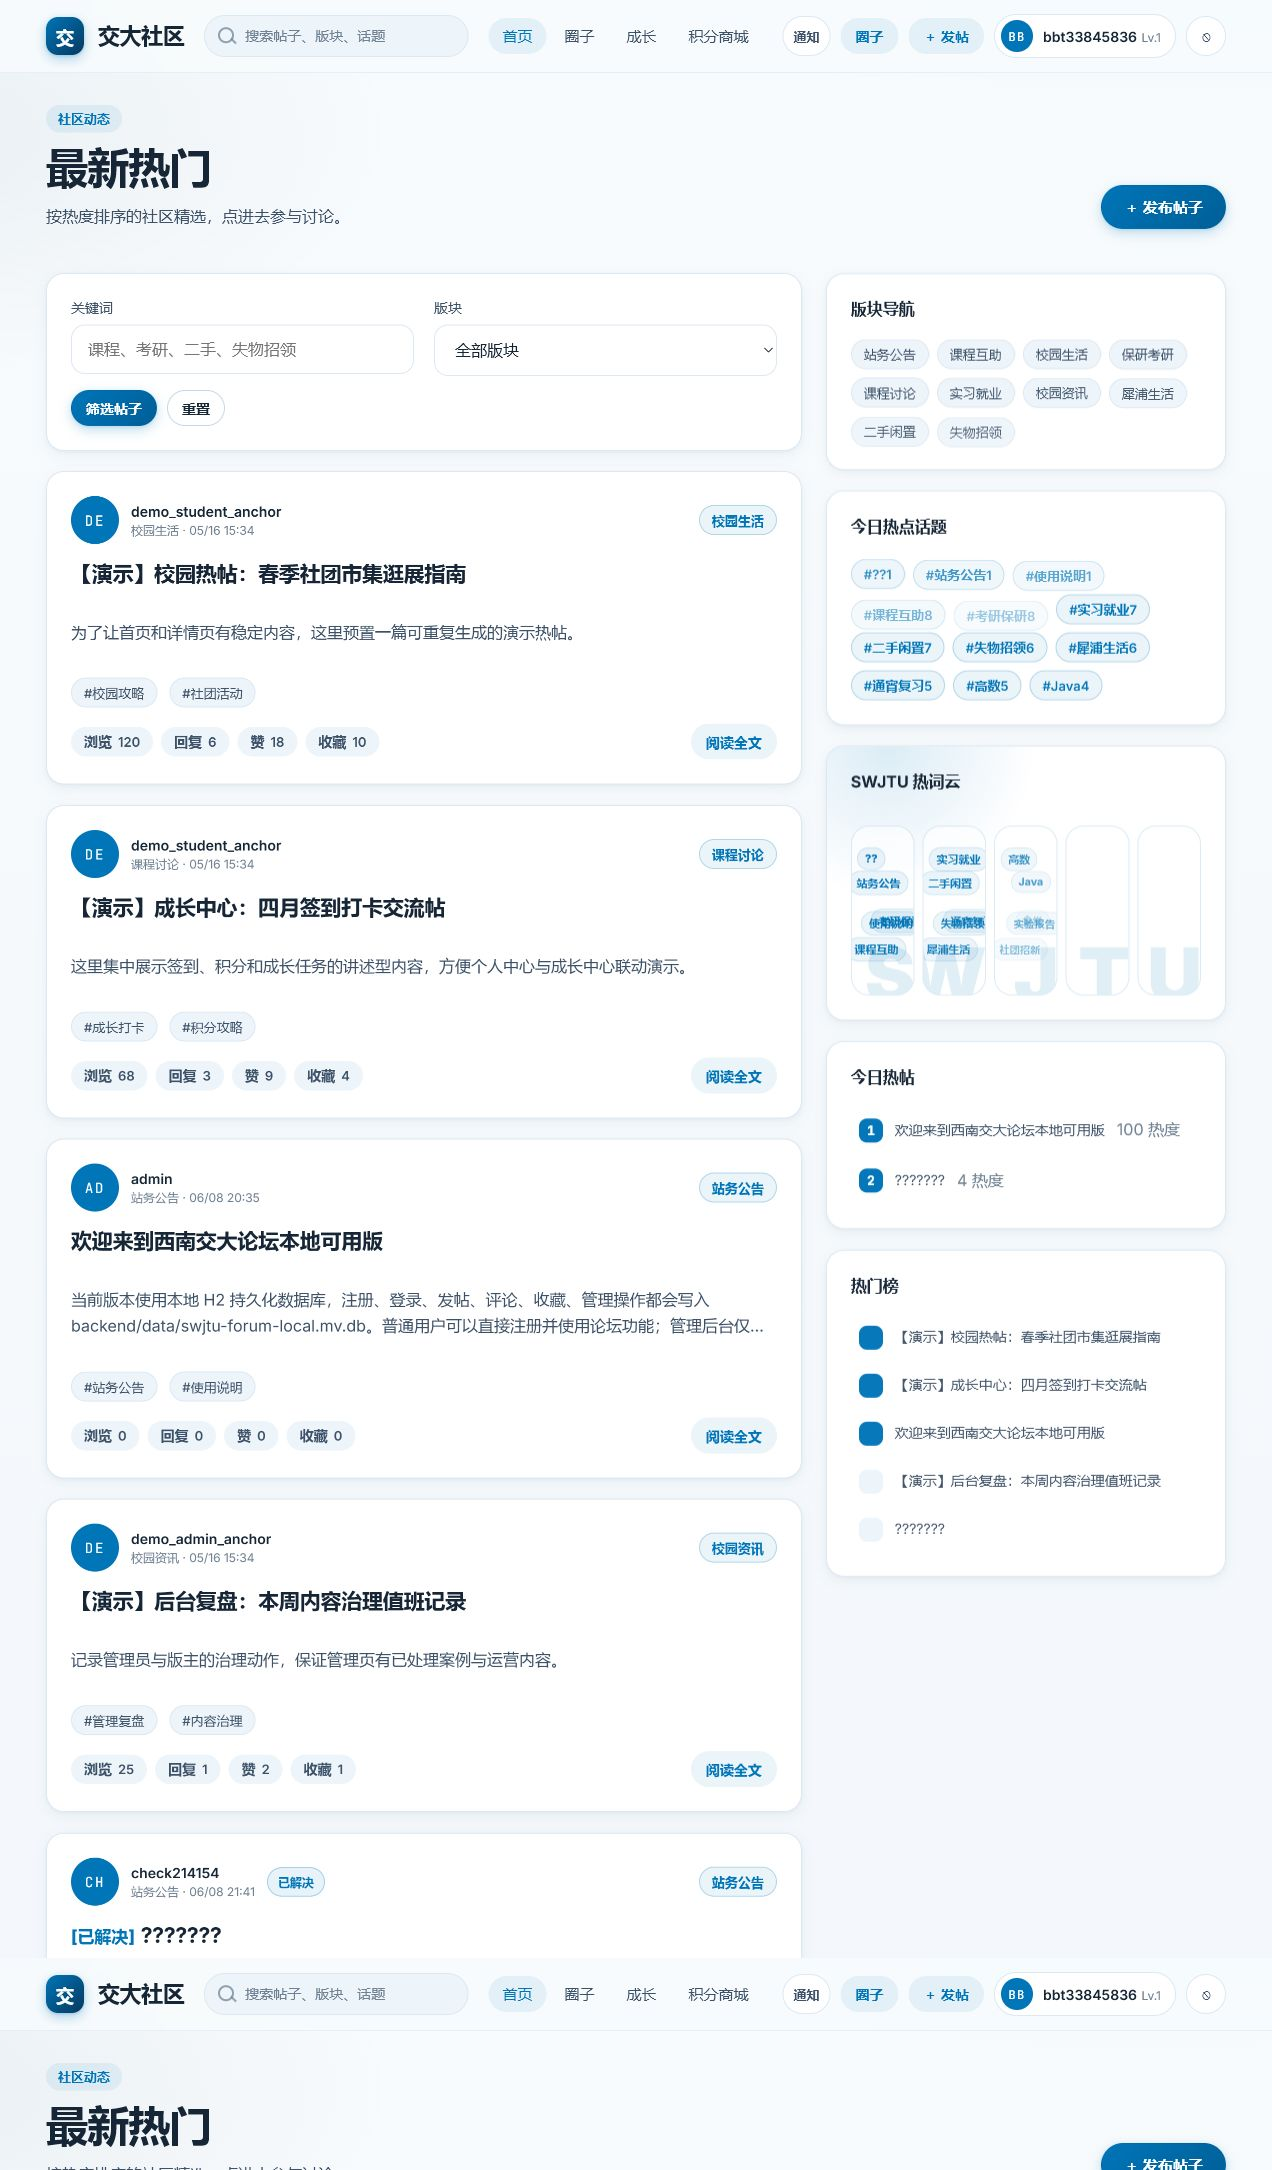
\includegraphics[width=0.88\textwidth]{figures/forum_test/05_home_post_list.png}
\caption{首页帖子列表截图}
\end{figure}
\begin{figure}[H]
\centering
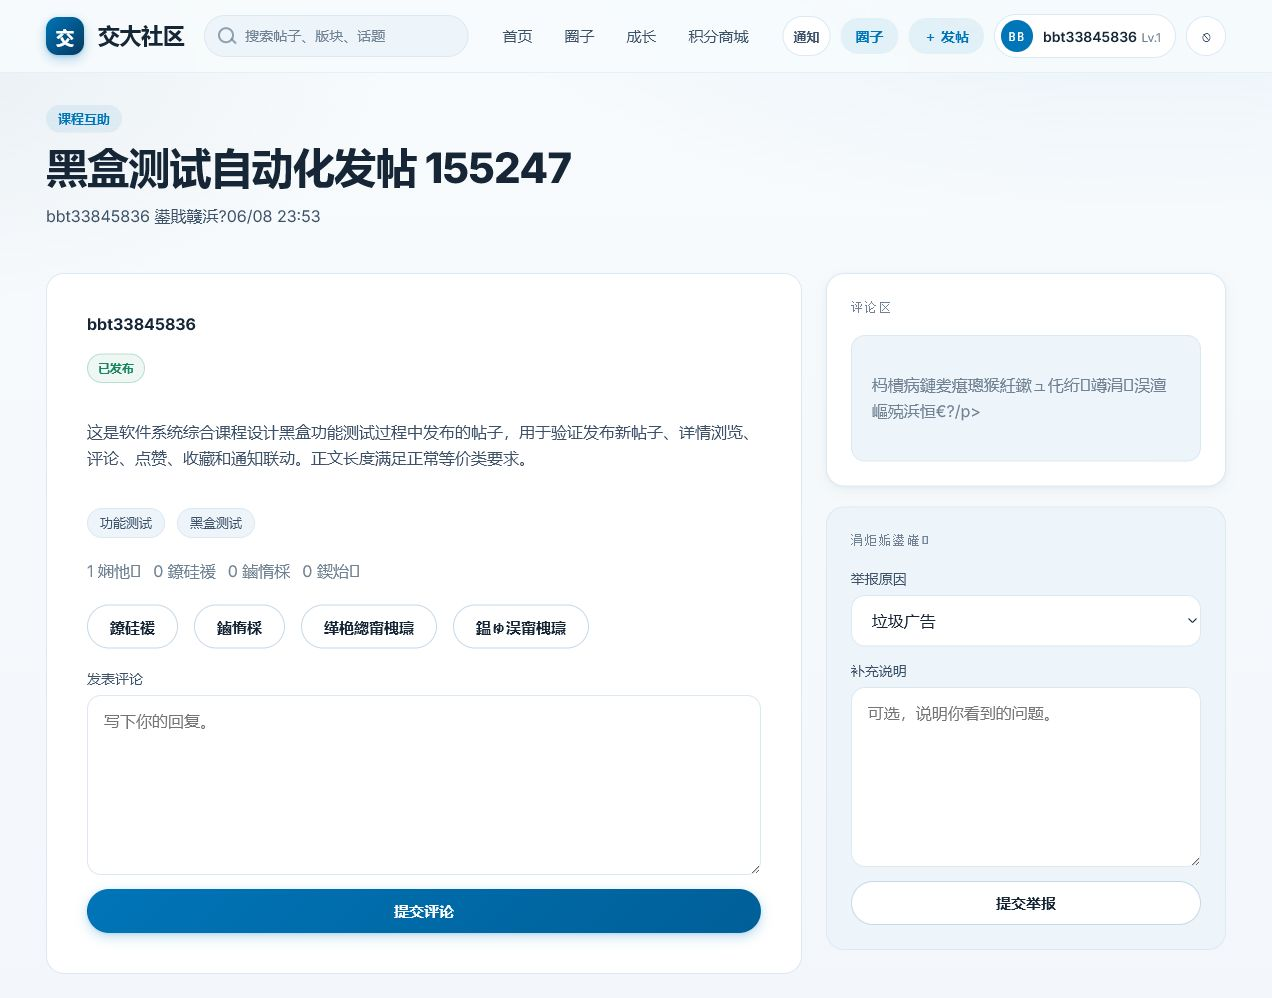
\includegraphics[width=0.88\textwidth]{figures/forum_test/09_create_post_success_detail.png}
\caption{发帖详情页截图}
\end{figure}
\begin{figure}[H]
\centering
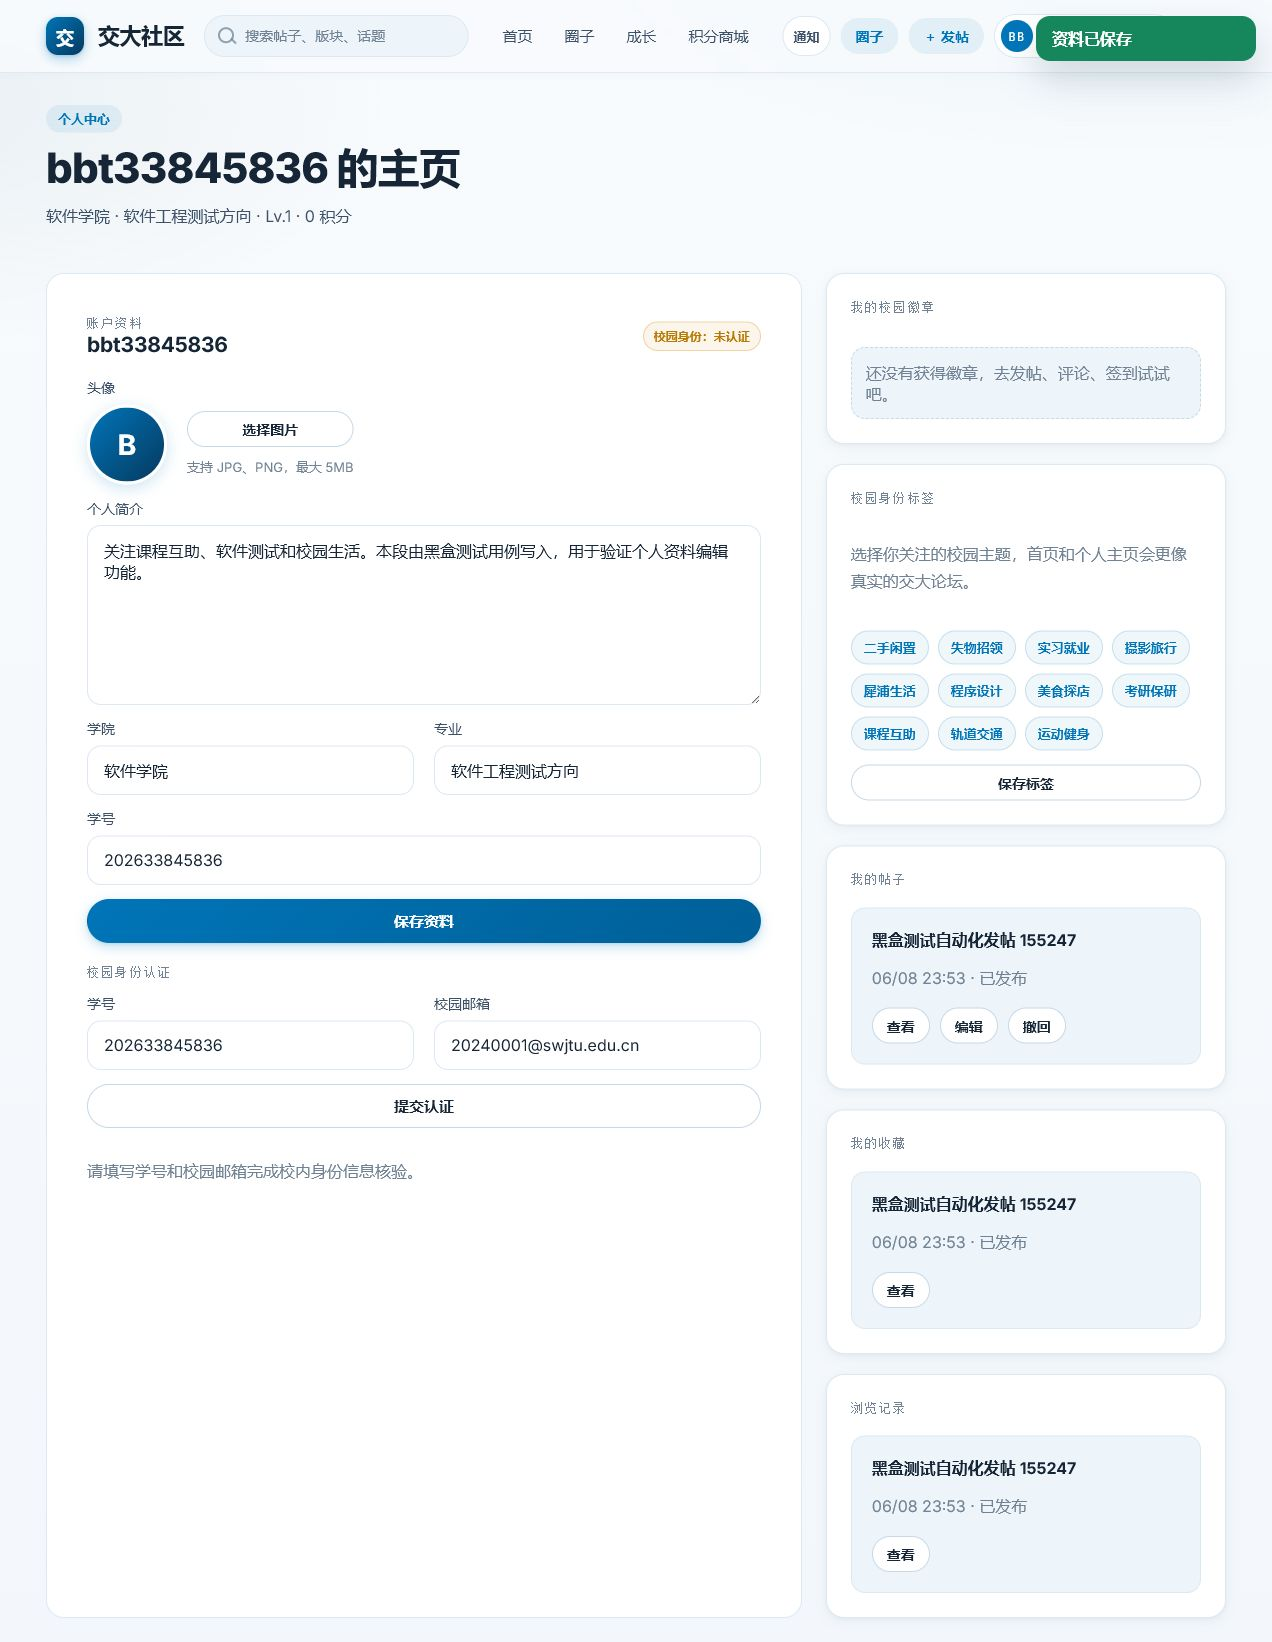
\includegraphics[width=0.88\textwidth]{figures/forum_test/14_profile_edit_success.png}
\caption{个人资料编辑成功截图}
\end{figure}
\begin{figure}[H]
\centering
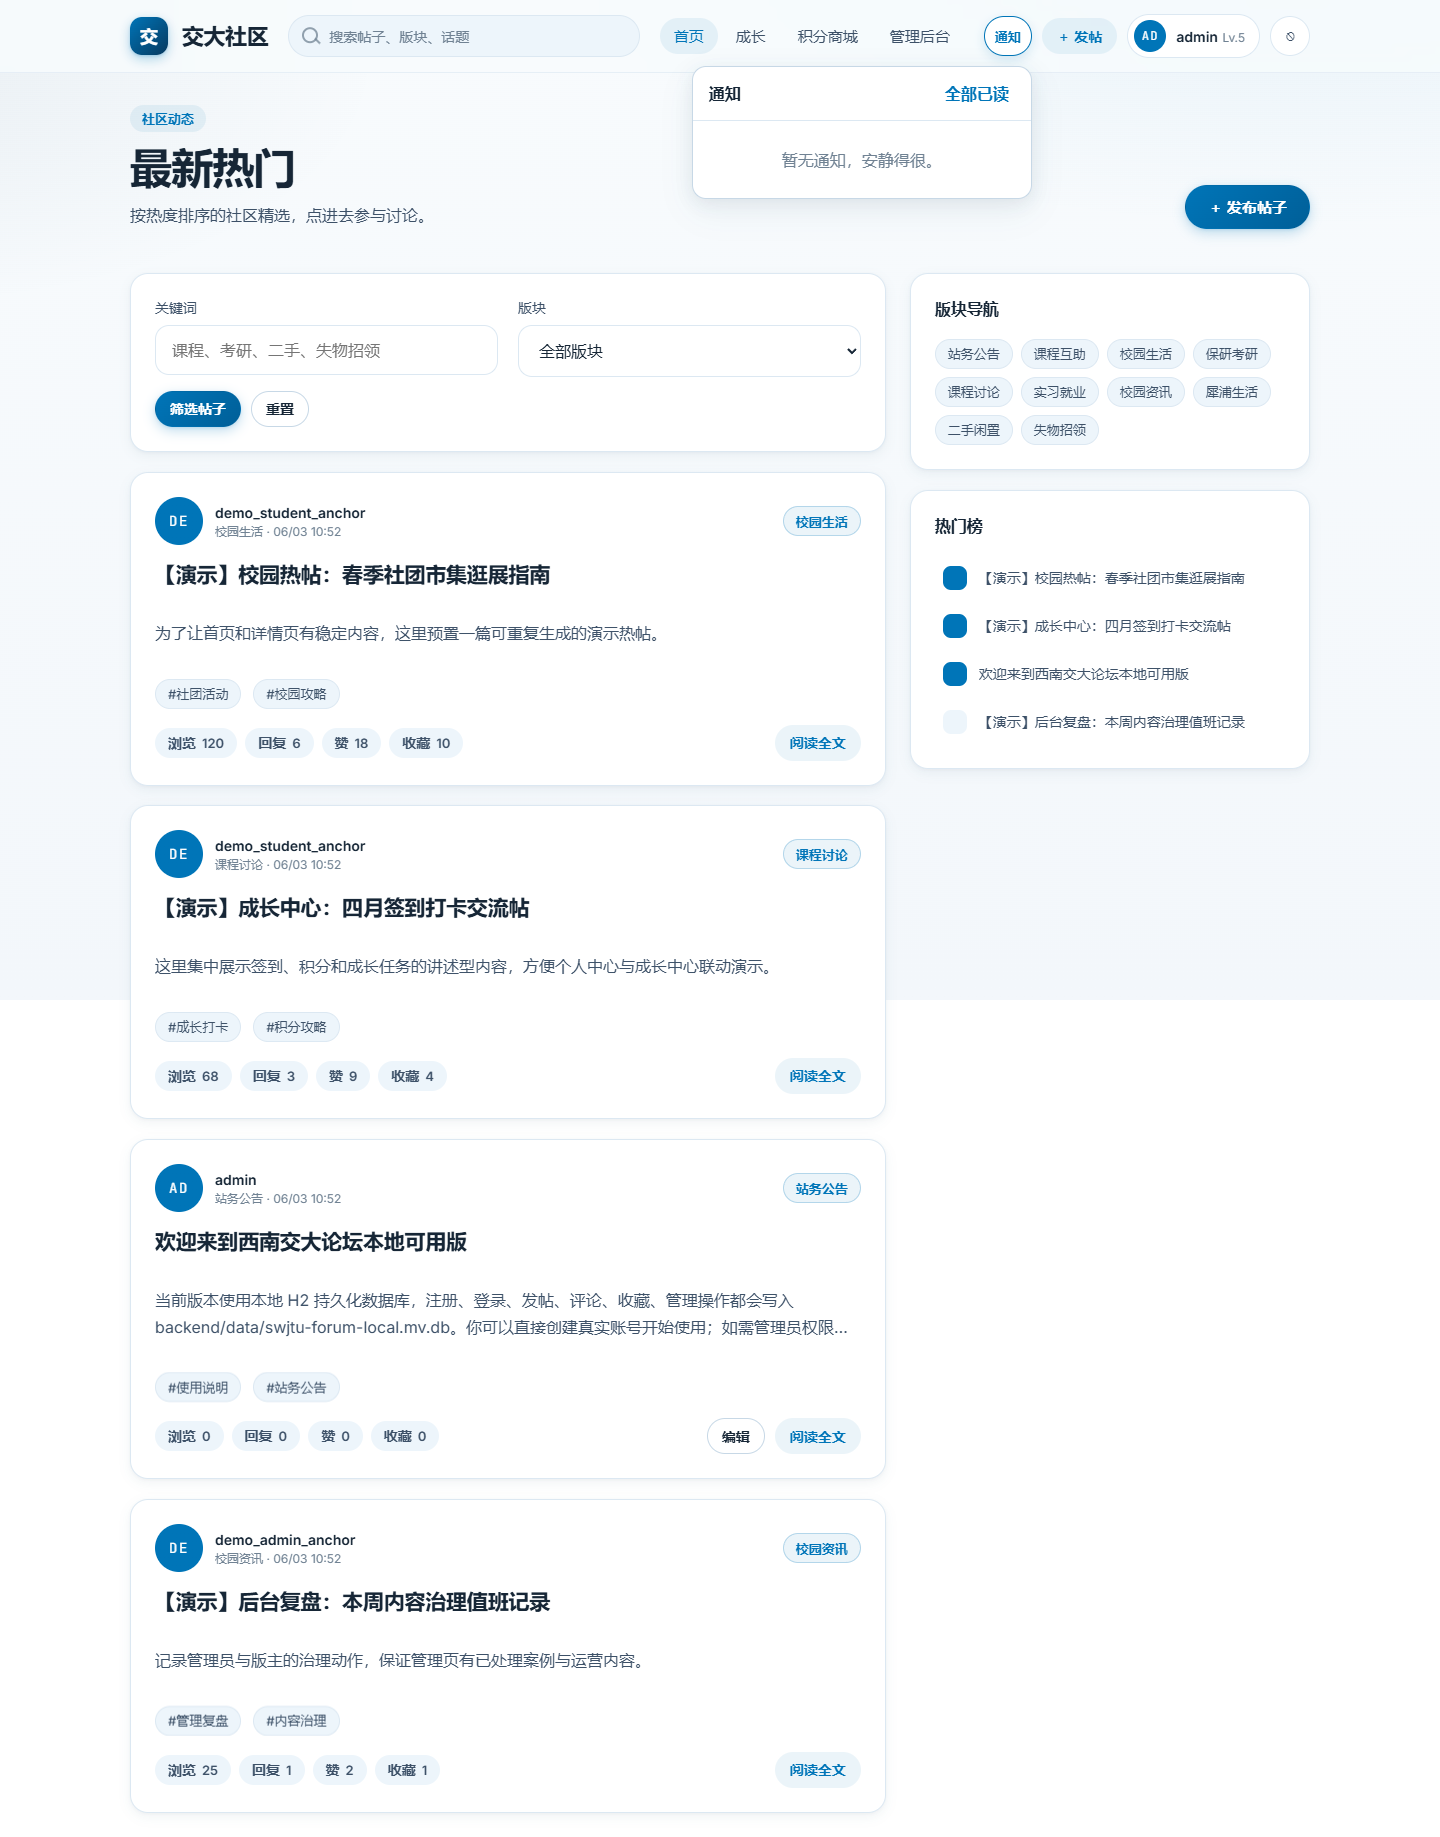
\includegraphics[width=0.88\textwidth]{figures/forum_test/BUG-001-notification-desktop.png}
\caption{通知中心桌面端修复后截图}
\end{figure}
\begin{figure}[H]
\centering
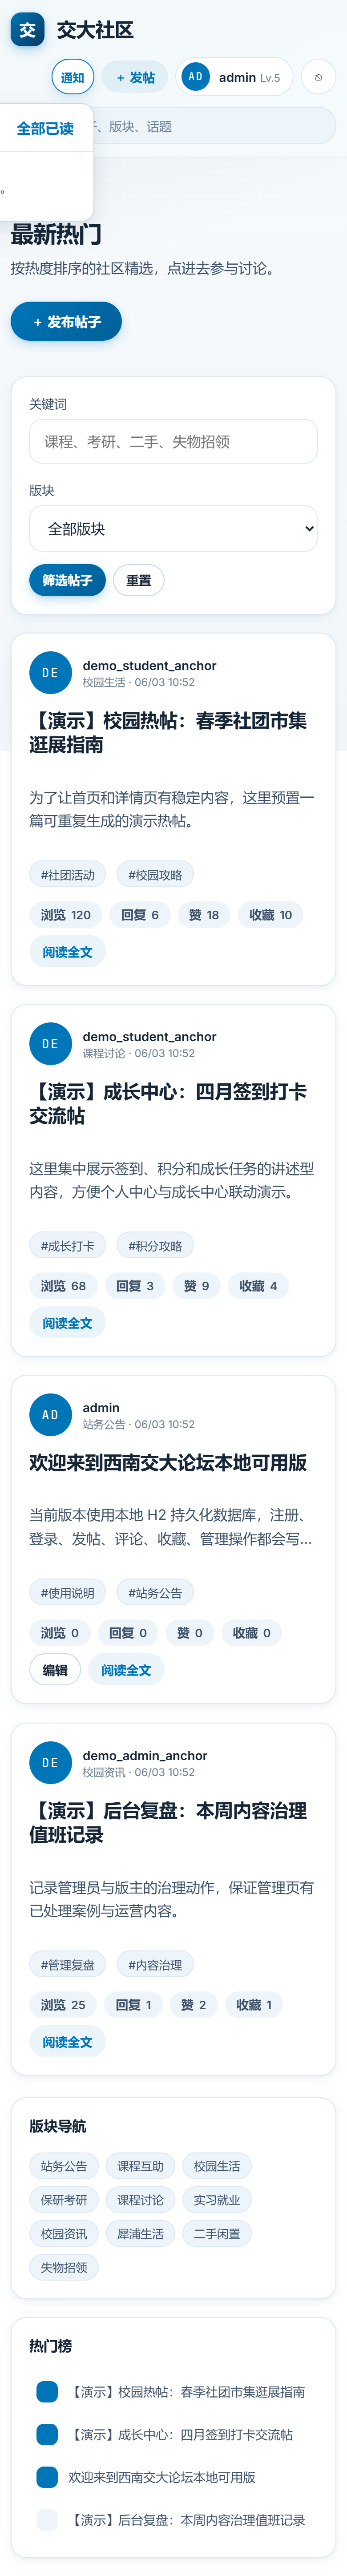
\includegraphics[width=0.88\textwidth]{figures/forum_test/BUG-001-notification-mobile.png}
\caption{通知中心移动端修复后截图}
\end{figure}
\begin{figure}[H]
\centering
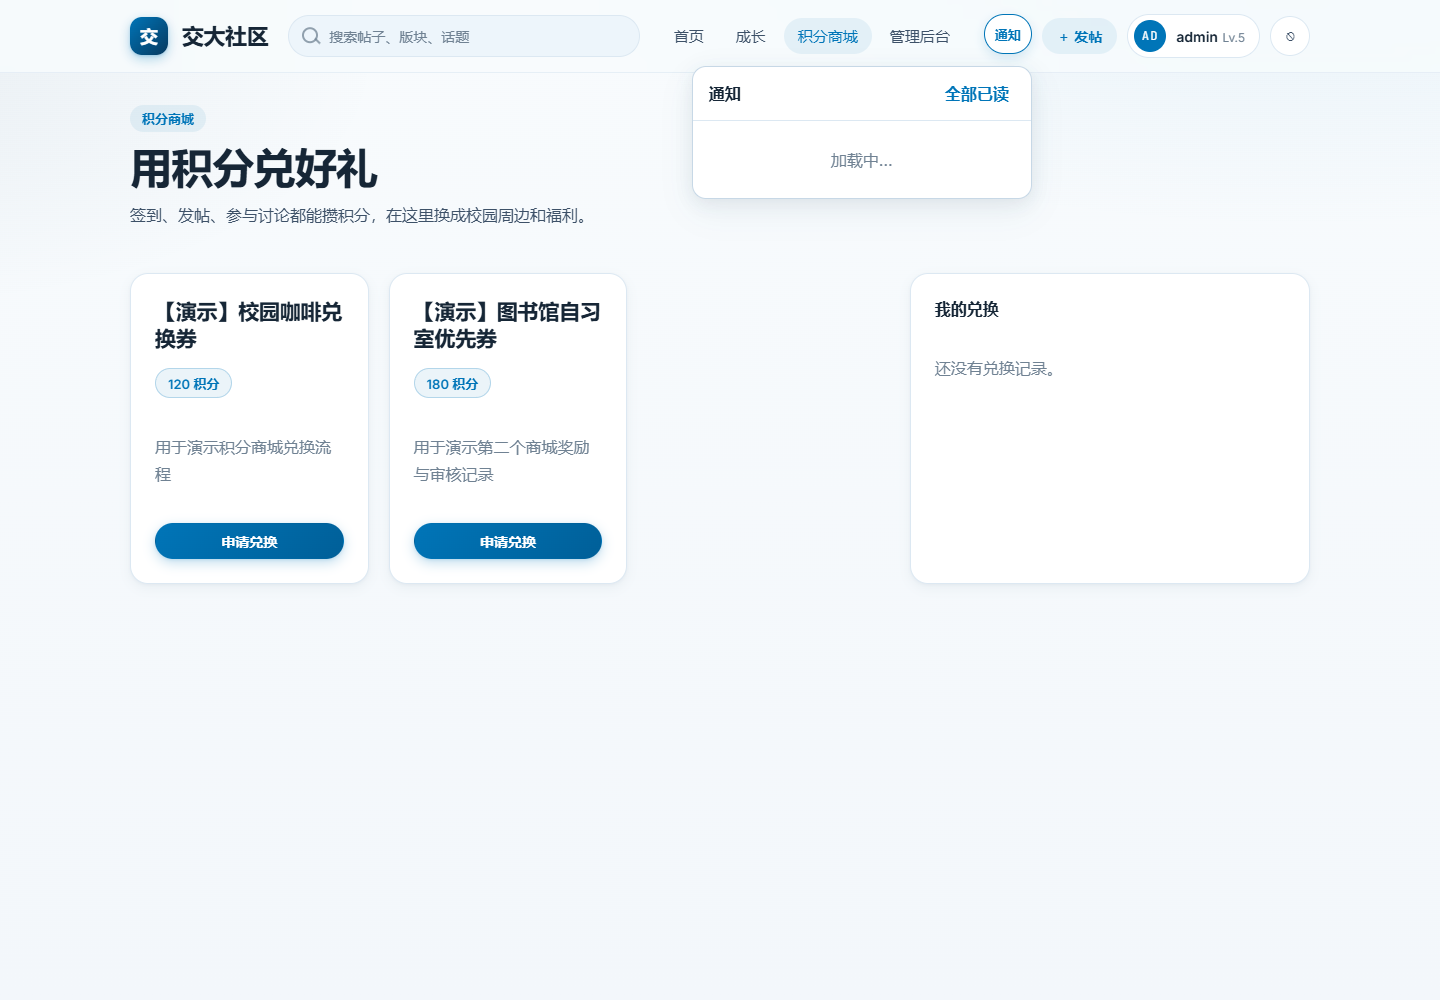
\includegraphics[width=0.88\textwidth]{figures/forum_test/BUG-002-rewards-redemptions.png}
\caption{积分商城兑换记录修复后截图}
\end{figure}
\begin{figure}[H]
\centering
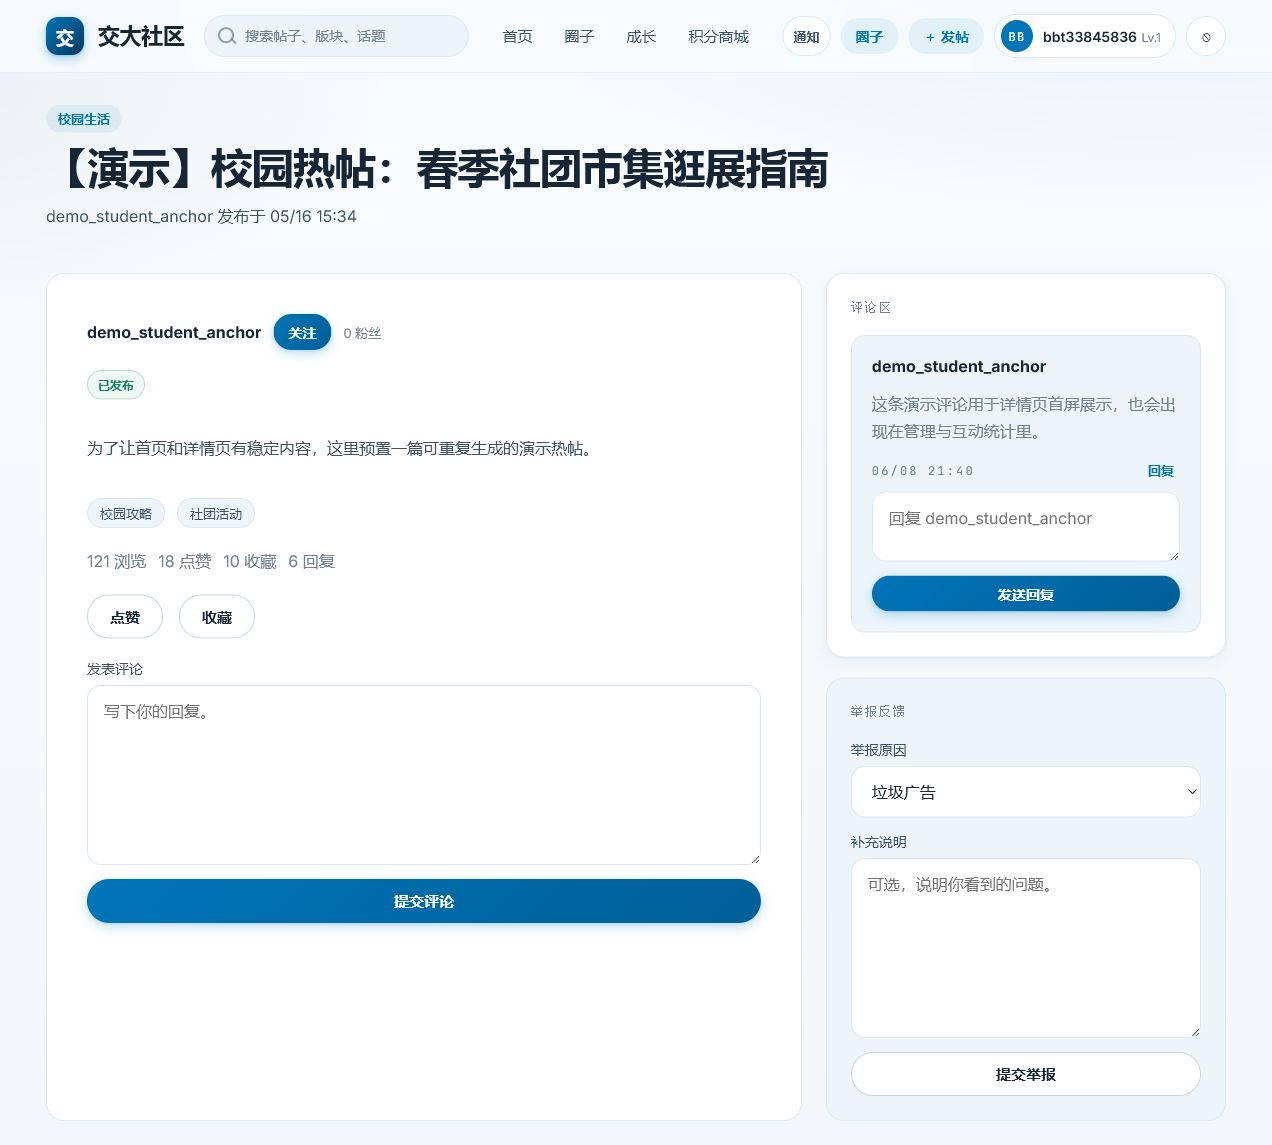
\includegraphics[width=0.88\textwidth]{figures/forum_test/23_follow_page_before.png}
\caption{关注功能页面截图}
\end{figure}

\section{缺陷清单}
\begin{longtable}{P{1.4cm}P{2.2cm}P{1.1cm}P{6.2cm}P{1.6cm}P{5.5cm}}
\toprule
编号 & 模块 & 严重 & 标题 & 状态 & 证据\\
\midrule
\endfirsthead
\toprule
编号 & 模块 & 严重 & 标题 & 状态 & 证据\\
\midrule
\endhead
BUG-001 & 通知中心 & 高 & 点击通知后面板DOM存在但不可见 & 已修复 & BUG-001-notification-desktop.png;BUG-001-notification-mobile.png \\
BUG-002 & 积分商城 & 高 & 兑换记录接口刷新出现500/页面加载失败 & 已修复 & BUG-002-rewards-redemptions.png;verification-summary.json \\
BUG-003 & 便携包启动 & 高 & 旧H2数据库升级comments.accepted非空列无默认值导致启动失败 & 已修复 & verification-summary.json \\
BUG-004 & 发帖 & 中 & 部分详情页按钮或静态文案出现中文乱码 & 待修复 & 09\_create\_post\_success\_detail.png \\
BUG-005 & 成长系统 & 中 & 签到记录区域积分展示与积分流水不完全一致 & 待修复 & 19\_daily\_checkin\_success\_or\_repeat.png \\
BUG-006 & 个人中心 & 低 & 校园身份认证覆盖学院专业前缺少二次确认 & 待优化 & 14\_profile\_edit\_success.png;15\_campus\_identity\_success.png \\
\bottomrule
\end{longtable}

\section{脚本开发遇到的问题与总结}
第一，纯Selenium点击所有场景较慢且容易受页面刷新影响，因此本轮将大部分可稳定验证的功能改为HTTP接口自动化执行，Selenium只用于关键页面与截图验证。第二，通知中心旧缺陷说明“DOM存在”不足以证明功能可用，因此脚本增加了hidden属性和computed display断言。第三，积分商城旧缺陷来自后端实体序列化，修复后使用DTO返回，并通过刷新页面和接口状态码双重回归。

本次压缩后的75条用例更贴近实际验收：每个功能点保留5条关键用例，覆盖主流程、异常、权限、状态和UI证据；低优先级和未验证设计项被删除，报告结果更真实、清晰，也更便于老师检查。
\end{document}
